
\documentclass[12pt]{article}

% Layout.
\usepackage[top=1.0in, bottom=0.75in, left=1in, right=1in, headheight=1.0in, headsep=0pt]{geometry}

% Fonts.
\usepackage{mathptmx}
\usepackage[scaled=0.86]{helvet}
\renewcommand{\emph}[1]{\textsf{\textbf{#1}}}

% TiKZ.
\usepackage{tikz, pgfplots}
\usetikzlibrary{calc}
\pgfplotsset{my style/.append style={axis x line=middle, axis y line=
middle, xlabel={$x$}, ylabel={$y$}, axis equal }}

% Misc packages.
\usepackage{amsmath,amssymb,latexsym, nicefrac}
\usepackage{graphicx}
\usepackage{array}
\usepackage{xcolor}
\usepackage{multicol}
\usepackage{adjustbox}


% Commands to set various header/footer components.
\makeatletter
\def\doctitle#1{\gdef\@doctitle{#1}}
\doctitle{Use {\tt\textbackslash doctitle\{MY LABEL\}}.}
\def\docdate#1{\gdef\@docdate{#1}}
\docdate{Use {\tt\textbackslash docdate\{MY DATE\}}.}
\def\doccourse#1{\gdef\@doccourse{#1}}
\let\@doccourse\@empty
\def\docscoring#1{\gdef\@docscoring{#1}}
\let\@docscoring\@empty
\def\docversion#1{\gdef\@docversion{#1}}
\let\@docversion\@empty
\makeatother

% Headers and footers layout.
\makeatletter
\usepackage{fancyhdr}
\pagestyle{fancy}
\fancyhf{} % Clears all headers/footers.
\lhead{\emph{\@doctitle\hfill\@docdate}
\ifnum \value{page} > 1\relax\else\\
\emph{Name: \rule{3.5in}{1pt}\hfill \@docscoring}
\\
%\emph{Circle one: \quad Rhodes (F01) \hskip 1ex\rule{1pt}{9pt}\hskip 1ex Bueler (F02)}
\fi}

\rfoot{\emph{\@docversion}}
\lfoot{\emph{\@doccourse}}
\cfoot{\emph{\thepage}}
\renewcommand{\headrulewidth}{0pt}%
\makeatother

% Paragraph spacing
\parindent 0pt
\parskip 6pt plus 1pt

% A problem is a section-like command. Use \problem{5} to
% start a problem worth 5 points.
\newcounter{probcount}
\newcounter{subprobcount}
\setcounter{probcount}{0}
\newcommand{\problem}[1]{%
\par
\addvspace{4pt}%
\setcounter{subprobcount}{0}%
\stepcounter{probcount}%
\makebox[0pt][r]{\emph{\arabic{probcount}.}\hskip1ex}\emph{[#1 points]}\hskip1ex}
\newcommand{\thesubproblem}{\emph{\alph{subprobcount}.}}

% Subproblems are an enumerate-like environment with a consistent
% numbering scheme. 
% Use \begin{subproblems}\item...\item...\end{subproblems}
\newenvironment{subproblems}{%
\begin{enumerate}%
\setcounter{enumi}{\value{subprobcount}}%
\renewcommand{\theenumi}{\emph{\alph{enumi}}}}%
{\setcounter{subprobcount}{\value{enumi}}\end{enumerate}}

% Blanks for answers in normal and math mode.
\newcommand{\blank}[1]{\rule{#1}{0.75pt}}
\newcommand{\mblank}[1]{\underline{\hspace{#1}}}
\def\emptybox(#1,#2){\framebox{\parbox[c][#2]{#1}{\rule{0pt}{0pt}}}}

% Misc.
\renewcommand{\d}{\displaystyle}
\newcommand{\ds}{\displaystyle}
\def\bc{\begin{center}}
\def\ec{\end{center}}

\newcommand{\ans}[1][2]{ \ \rule{#1 in}{.5 pt} \ }


\doctitle{Math 251: Quiz 9}
\docdate{November 19, 2019}
\doccourse{UAF Calculus I}
\docversion{v-2}
\docscoring{{\Large \strut}\blank{0.8in} / 25}

\begin{document}
25 points possible.  No aids (book, calculator, etc.) are permitted.  You need not simplify unless asked, but show all work and use proper notation for full credit.

\problem{5} Oil leaked out from a tanker at a rate of $r(t)$ liters per hour (L/h). Every two hours, the rate of flow out of the tanker was measured as shown in the table. Estimate the total amount of oil that leaked from the tanker over the 8 hours.  Include units in your answer.

\begin{center}
\begin{tabular}{l | c c c c c}
$t$ (in hours) & 0 & 2 & 4 & 6 & 8\\ \hline
$r(t)$ (in liters/hour) & 0 & 5 & 10 & 15 & 25
\end{tabular}
\end{center}
\vspace{1.5in}

\problem{6}  

%\begin{adjustbox}{valign=t,minipage={.45\textwidth}}

Given $f(x) = \frac{1}{1+x}$, approximate the area (shaded in gray) bounded between the curve and the $x$-axis and the lines $x = 1$ and $x= 3$ using \fbox{three {\sc left-hand} rectangles}.  {\bf Draw and shade in the rectangles you are using on the graph.} Show your computation clearly. You do not need to simplify your answer.
%, and simplify your answer.

%\end{adjustbox}
%
\begin{adjustbox}{valign=t,minipage={.55\textwidth}}
(a) Width of each rectangle = \ans[.5] 
\end{adjustbox}
\begin{adjustbox}{valign=t,minipage={.35\textwidth}}
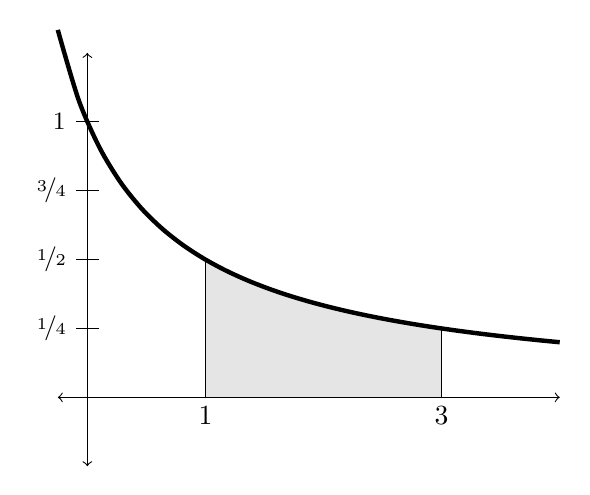
\begin{tikzpicture}[xscale = 1.5,yscale=3.5]
\fill [gray!20, domain=1:3, variable=\x]
  (1, 0)
  -- plot ({\x}, {1/(1+\x})
  -- (3, 0)
  -- cycle;
  \draw[ultra thick, ] plot[smooth, domain=-.25:4]({\x,1/(1+\x)});
\draw (1, 1/2)--(1,0) node[below] {1};
\draw (3, 1/4) -- (3,0)node[below] {3};
\draw[<->] (-.25,0) -- (4,0);
\draw[<->] (0,-.25) -- (0, 1.25);
\draw (.1, 1/2)-- (-.1, 1/2) node[left]{{\small $\nicefrac{1}{2}$}} ;
\draw (.1, 1/4)-- (-.1, 1/4) node[left]{{\small $\nicefrac{1}{4}$}} ;
\draw (.1, 3/4)-- (-.1, 3/4) node[left]{{\small $\nicefrac{3}{4}$}} ;
\draw (.1, 1)-- (-.1, 1) node[left]{{\small 1}} ;


\end{tikzpicture}
\end{adjustbox}

\vfill
%(b) Approximate area = \ans

(b) Is your answer an overestimate or an underestimate for the actual area, and why? \\

\hrulefill

%\end{adjustbox}

%\vspace{10mm}

% 
\newpage
\problem{3} [Fill in the blank.] Using the graph of $f(x)$ shown to the right and  geometry, calculate exactly each of the following quantities:

\begin{adjustbox}{valign=t,minipage={.45\textwidth}}
\begin{subproblems}
\item $\d \int_{-2}^{0} f(x) \ dx$ = \ans[.5]
\vspace{.5in}

\item $\d \int_{2}^{4} f(x) \ dx$ = \ans[.5]
\vspace{.5in}

\item $\d \int_{1}^{6} f(x) \ dx$ = \ans[.5]
\vspace{.5in}

\end{subproblems}
\end{adjustbox}
%
\begin{adjustbox}{valign=t,minipage={.45\textwidth}}
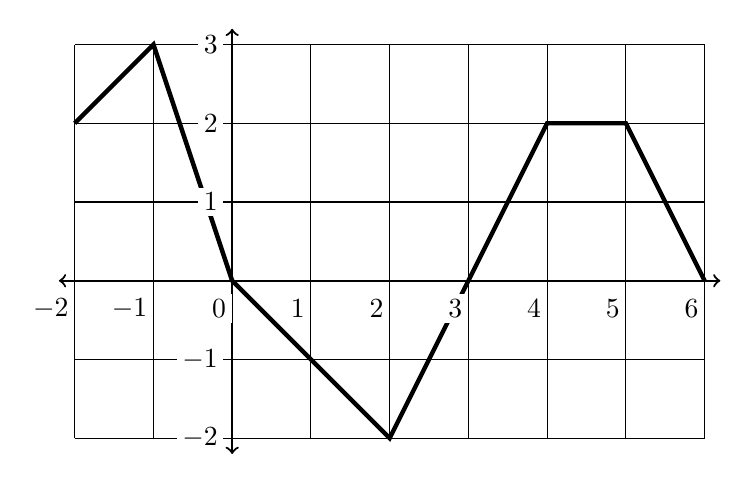
\begin{tikzpicture}[scale=1]
\draw[thin] (-2,-2) grid (6,3);
\draw[<->, thick] (-2.2,0) -- (6.2,0);
\draw[<->, thick] (0,-2.2) -- (0, 3.2);
%\draw[ultra thick] (-2,0) -- (-1,2) -- (0,2) -- (2,-2) -- (4,0)  --(5,3)-- (6,2);
\draw[ultra thick] (4+2,0) -- (4+1,2) -- (4-0,2) -- (4-2,-2) -- (4-4,0)  --(4-5,3)-- (4-6,2);
\foreach \i in {-2, -1,1,2, 3}{\draw (0,\i) node[left=3 pt,fill=white, inner sep=2pt] {$\i$};}
\foreach \i in {-2, -1,0,1,2, 3,4,5,6}{\draw (\i,0) node[below=10pt, left= .01 pt, fill=white, inner sep=2pt] {$\i$};}

\end{tikzpicture}
\end{adjustbox}


\problem{8} [Fill in the blank.] If $\d \int_{1}^{5} f(x) \ dx = 5$, $\d \int_{1}^{8} f(x) \ dx = 8$ and $\d \int_{1}^{5} g(x) \ dx = -3$, compute the following quantities:

\begin{subproblems}
\item $\d \int_{1}^{5} 3 f(x) \ dx = $ 

\item $\d \int_{1}^{5} 2 f(x) - 6 \ dx = $ %2pt

\item $\d \int_{3}^{3} g(x) \ dx = $

\item  $\d \int_{1}^{5} f(x) - 2 g(x) \ dx = $

\item  $\d \int_{5}^{1} f(x) \ dx = $

\item $\d \int_{5}^{8} f(x) \ dx = $ %2 pt
\end{subproblems}

\problem{3} Use geometry to determine $\d \int_{-4}^{0} \sqrt{16-x^{2}} \ dx$. Justify your answer with a few words or a sketch.

\vspace{1in}





\end{document}